\documentclass{article}
\usepackage[a4paper,left=3cm,right=3cm,top=3cm,bottom=3cm]{geometry}
\usepackage[utf8]{inputenc}
\usepackage[T1]{fontenc}
\usepackage{latexsym,amsfonts,amsmath,amssymb,amstext,graphicx,titlesec,ae,aecompl,mathtools,tabularx, multirow, cancel, nicefrac,subcaption, blindtext, floatrow}
\setlength{\parindent}{0pt}
\newfloatcommand{capbtabbox}{table}[][\FBwidth]


\begin{document}

\begin{titlepage}
       \begin{center}
             \begin{huge}
				   %% Update assignment number here
                   \textbf{Assignment 3}
             \end{huge}
       \end{center}

       \begin{center}
             \begin{large}
                   Computational Intelligence, SS2020
             \end{large}
       \end{center}

       \begin{center}
 \begin{tabularx}{\textwidth}{|>{\hsize=.33\hsize}X|>{\hsize=.33\hsize}X|>{\hsize=.33\hsize}X|} 

                   \hline
                   \multicolumn{3}{|c|}{\textbf{Team Members}} \\
                   \hline
                   Last name & First name & Matriculation Number \\
                   \hline
                   Blöcher & Christian & 01573246 \\
                   \hline
                   Bürgener & Max & 01531577 \\
                   \hline
                    &  &  \\
                   \hline

             \end{tabularx}
       \end{center}
\end{titlepage}

\section{Regression with Neural Networks}
\subsection{Simple Regression with Neural Networks}
\subsubsection{Learned Function}


\subsubsection{Variability of the performance of deep neural networks}


\subsubsection{Varying the number of hidden neurons}


\subsubsection{Change of MSE during the course of training}

\clearpage
\subsection{Regularized Neural Networks: Weight Decay}

\newpage

\clearpage
\section{Classification with Neural Networks: Fashion MNIST}

\begin{itemize}
	\item The confusion matrix
	
	\begin{table}[!ht]
        \begin{tabular}{|l|c|c|c|c|c|c|c|c|c|c|}
        \hline
                  & T-Shirt/top & Trousers & Pullover & Dress & Coat & Sandal & Shirt & Sneaker & Bag & Ankle boot \\ \hline
      T-Shirt/top & 841         & 3        & 12       & 25    & 4    & 1      & 108   & 0       & 6   & 0          \\ \hline
      Trousers    & 7           & 960      & 2        & 21    & 5    & 0      & 4     & 0       & 1   & 0          \\ \hline
      Pullover    & 19          & 0        & 835      & 15    & 52   & 0      & 78    & 0       & 1   & 0          \\ \hline
      Dress       & 21          & 4        & 14       & 904   & 23   & 0      & 31    & 0       & 3   & 0          \\ \hline
      Coat        & 2           & 1        & 104      & 30    & 797  & 0      & 65    & 0       & 1   & 0          \\ \hline
      Sandal      & 1           & 0        & 0        & 1     & 0    & 955    & 0     & 23      & 2   & 18         \\ \hline
      Shirt       & 104         & 1        & 75       & 26    & 45   & 1      & 741   & 0       & 7   & 0          \\ \hline
      Sneaker     & 0           & 0        & 0        & 0     & 0    & 15     & 0     & 958     & 0   & 27         \\ \hline
      Bag         & 5           & 0        & 5        & 6     & 2    & 3      & 4     & 4       & 970 & 1          \\ \hline
      Ankle boot  & 1           & 0        & 0        & 0     & 0    & 9      & 0     & 3       & 0   & 960        \\ \hline
        \end{tabular}
        \caption{Confusion matrix for Fashion MNIST Classification}
        \end{table}
       
        The rows of our confusion matrix correspond to the true classes and the columns to the predicted classes. The global accuracy for all classes is fairly good with $89,2\%$. Apparently it was difficult for the code to distinguish t-shirts/tops from shirts and coats from pullovers. Also remarkable is that all top clothes were often mistakenly recognized as shirts.\\
      
    \item Are particular regions of the images get more weights than others?
      
        \begin{figure}[!ht]
		\centering
		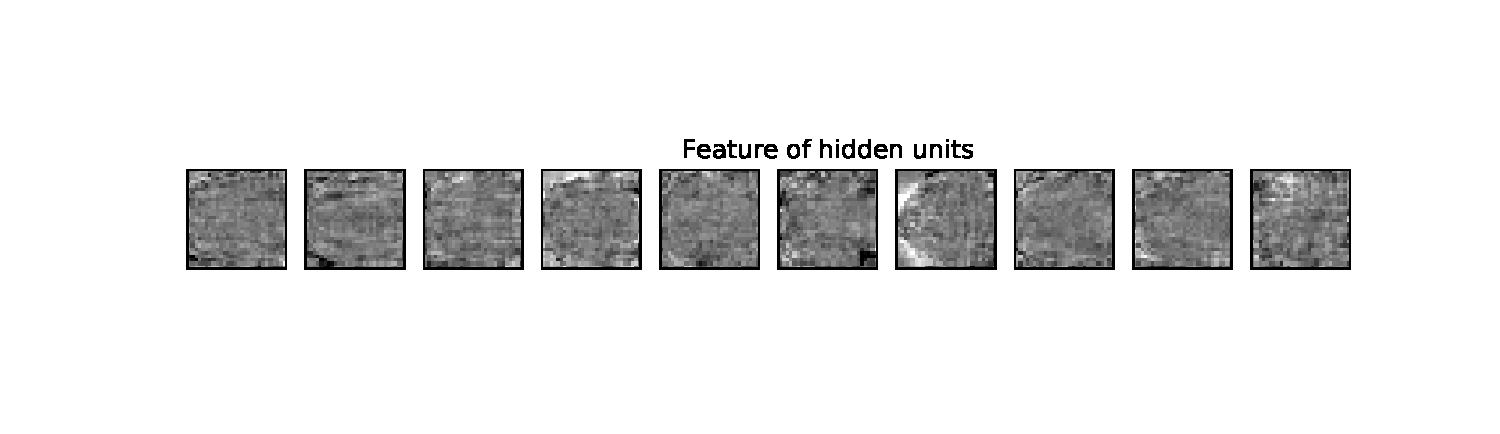
\includegraphics[width=1.2 \textwidth]{./Figures/2_weights.pdf}
		\caption{Weights per pixel for 10 samples}
		\label{weights}
		\end{figure}
	
	    In figure \ref{weights} are the weights per features visualized. As for the features these are referring to one pixel of a 28 x 28 pixel conversion from each picture. The weights are scaled from important regions (white) to regions with less information (black). It makes sense and can be seen in the pictures that that the object edges are important since all picture have the black background in common and the object outlines vary a lot.
	  
	\newpage    
    \item Boxplot of classifications with different inital weight vector values
    
        \begin{figure}[!ht]
		\centering
		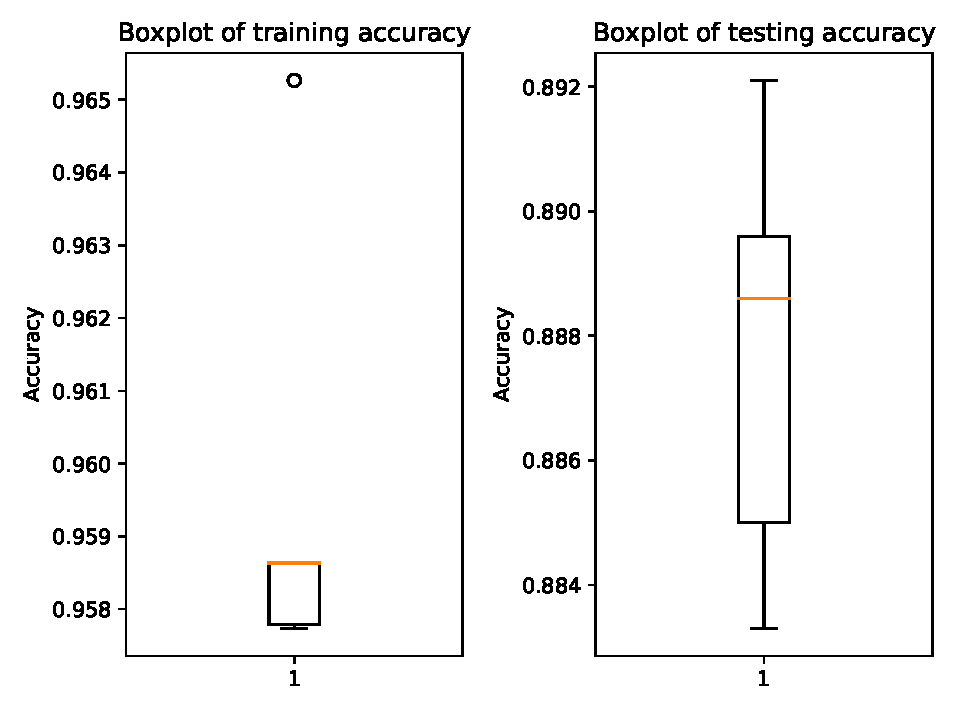
\includegraphics[width=1 \textwidth]{./Figures/2_1_boxplot.pdf}
		\caption{Accuracy of classifications using different inital $\mathbf{w}$}
		\label{weights}
		\end{figure}
		
		After choosing the optimal amount of hidden layers the boxplots visualize the accuracy of classifications which started with different weight vectors $\mathbf{w}$. The orange coloured line shows the median of our calculated numbers. The lower border of the box is enclosing the median of all numbers which are lower than our global median. The upper border is enclosing all numbers till the median of all higher numbers. The last section is showing the global minimum and maximum. Any outliers are marked with a spot.\\
		
	\item Missclassified items
	
\begin{figure}[!ht]
\centering
\makebox[\textwidth]{
\begin{subfigure}{0.5\textwidth}
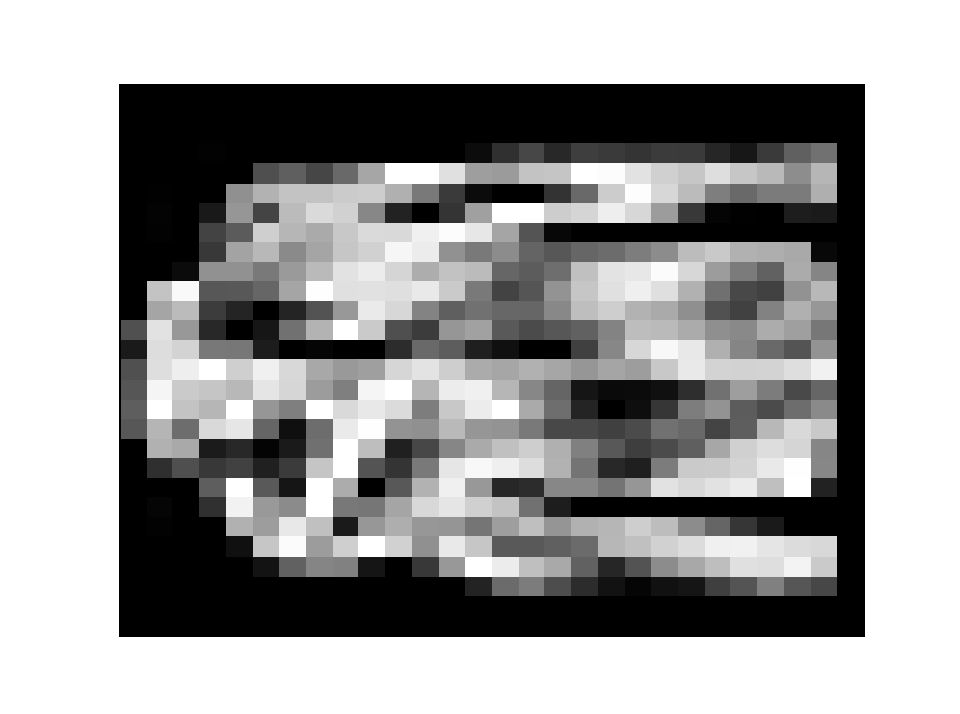
\includegraphics[width=\textwidth]{./Figures/2_misclassified_1.pdf}
\caption{Missclassified image 1}
\end{subfigure}
\begin{subfigure}{0.5\textwidth}
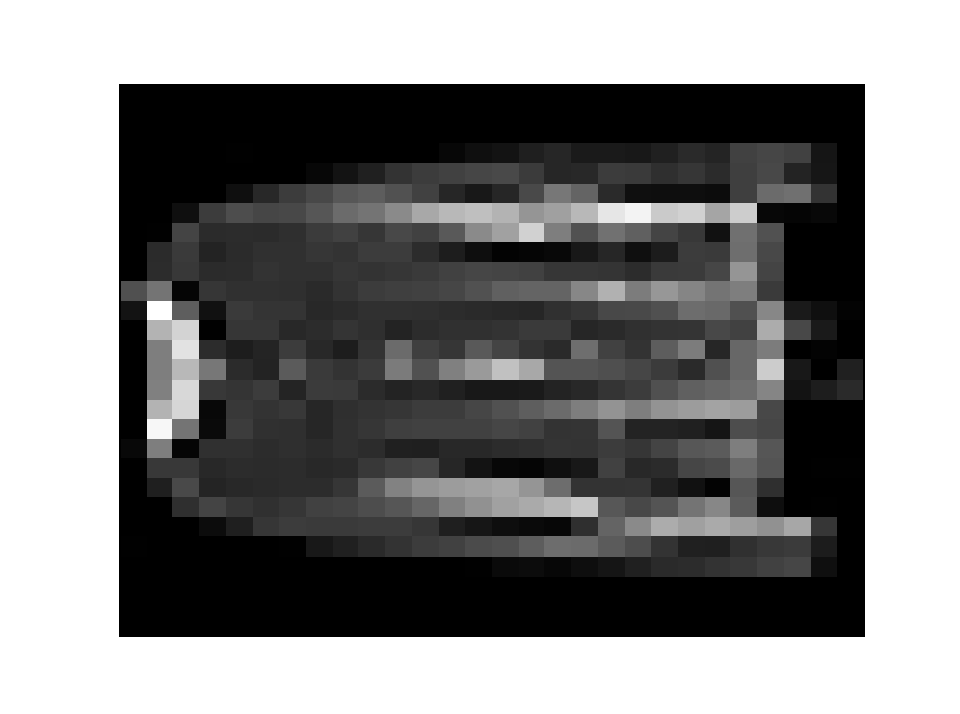
\includegraphics[width=\textwidth]{./Figures/2_misclassified_3.pdf}
\caption{Missclassified image 2}
\end{subfigure}
}

\makebox[\textwidth]{
\begin{subfigure}{0.5\textwidth}
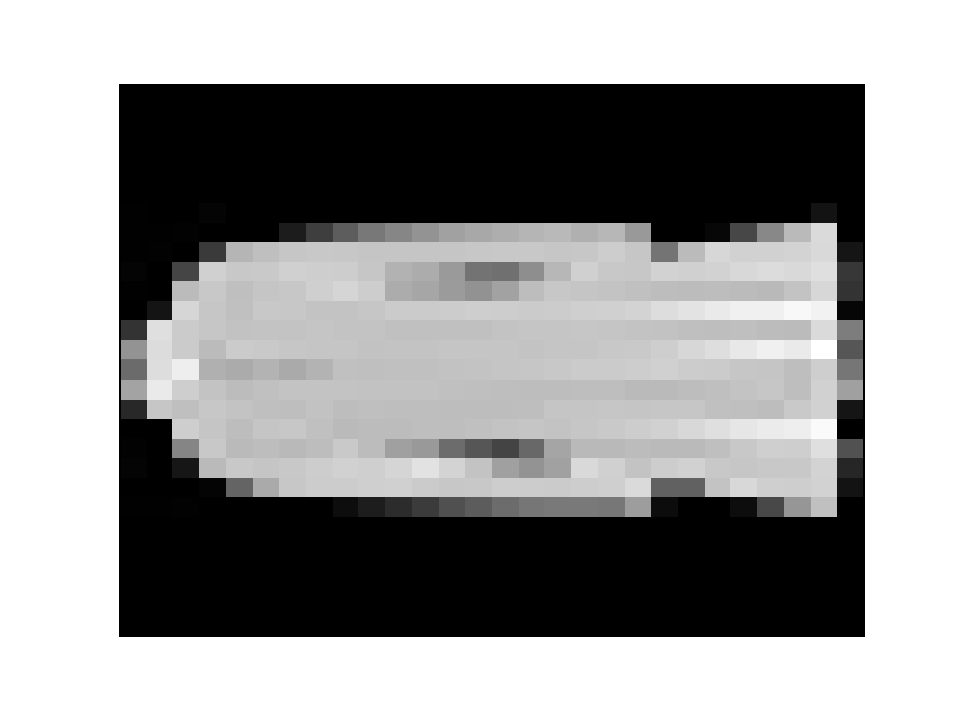
\includegraphics[width=\textwidth]{./Figures/2_misclassified_4.pdf}
\caption{Missclassified image 3}
\end{subfigure}
\begin{subfigure}{0.5\textwidth}
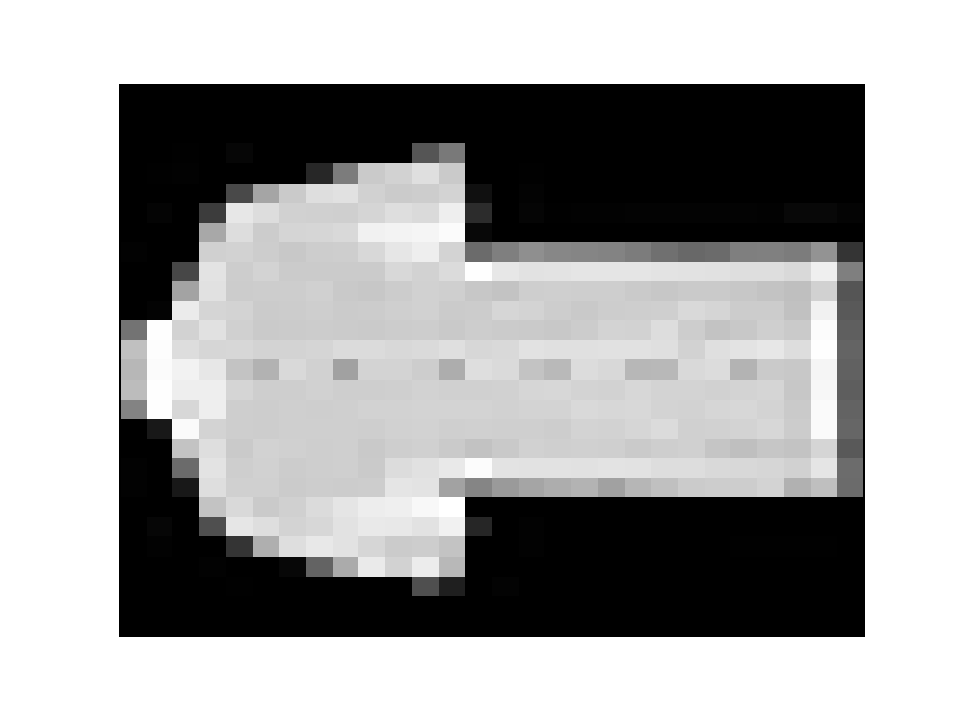
\includegraphics[width=\textwidth]{./Figures/2_misclassified_5.pdf}
\caption{Missclassified image 4}
\end{subfigure}
}
\caption{Missclassified items from our test set}
\label{linreg_poly1}
\end{figure}

\end{itemize}

\newpage
\clearpage
\section{Bonus: Implementation of a Perceptron}

\begin{itemize}
	\item Linear separable dataset:
	
	\begin{figure}[!ht]
	\makebox[\textwidth]{
	\begin{subfigure}{0.45\textwidth}
	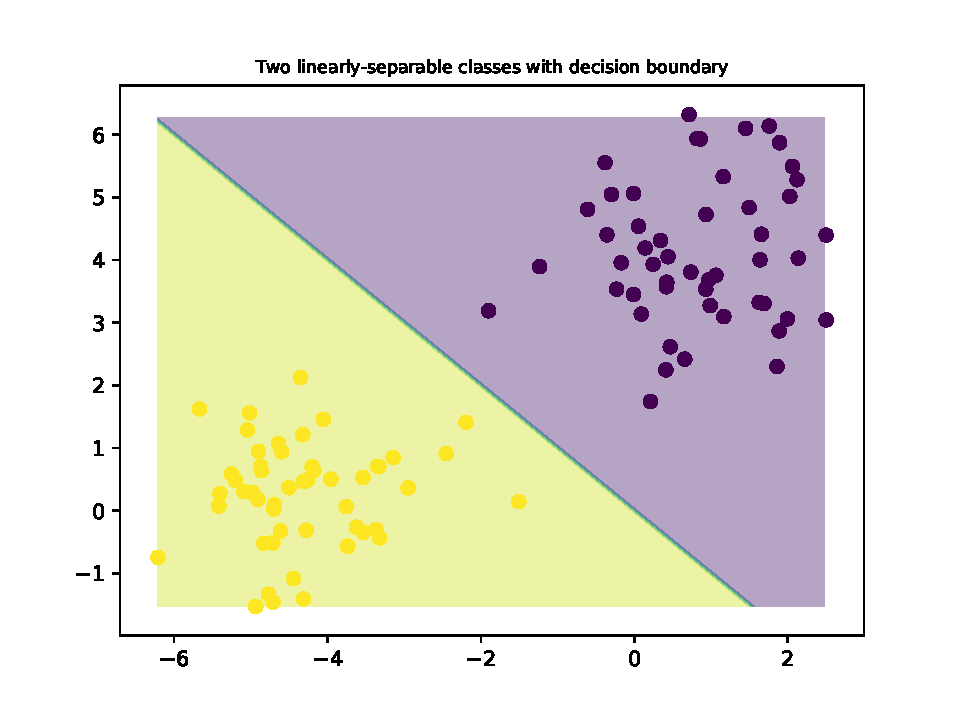
\includegraphics[width=\textwidth]{./Figures/3_lin_eta001_iter1.pdf}
	\caption{self implementation}
	\end{subfigure}
	\begin{subfigure}{0.45\textwidth}
	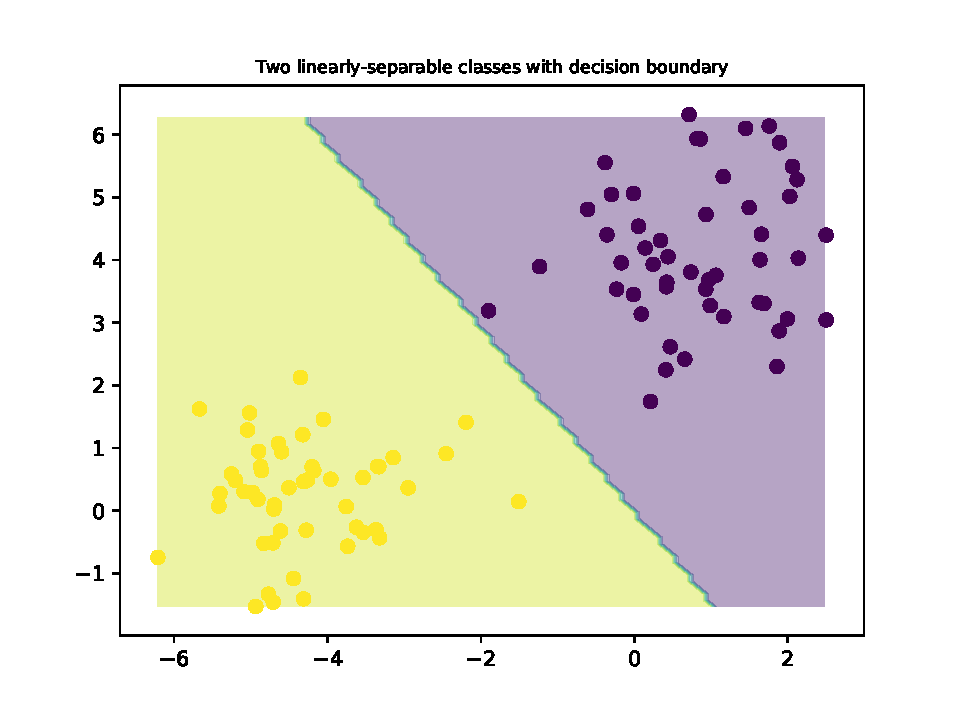
\includegraphics[width=\textwidth]{./Figures/3_lin_eta001_iter1_skl.pdf}
	\caption{scikit-learn’s implementation}
	\end{subfigure}
	}	
	\caption{Classification using eta = $0,01$ and max. iterations of 2}
	\label{perceptron1}
	\end{figure}
	
	\begin{figure}[!ht]
	\makebox[\textwidth]{
	\begin{subfigure}{0.45\textwidth}
	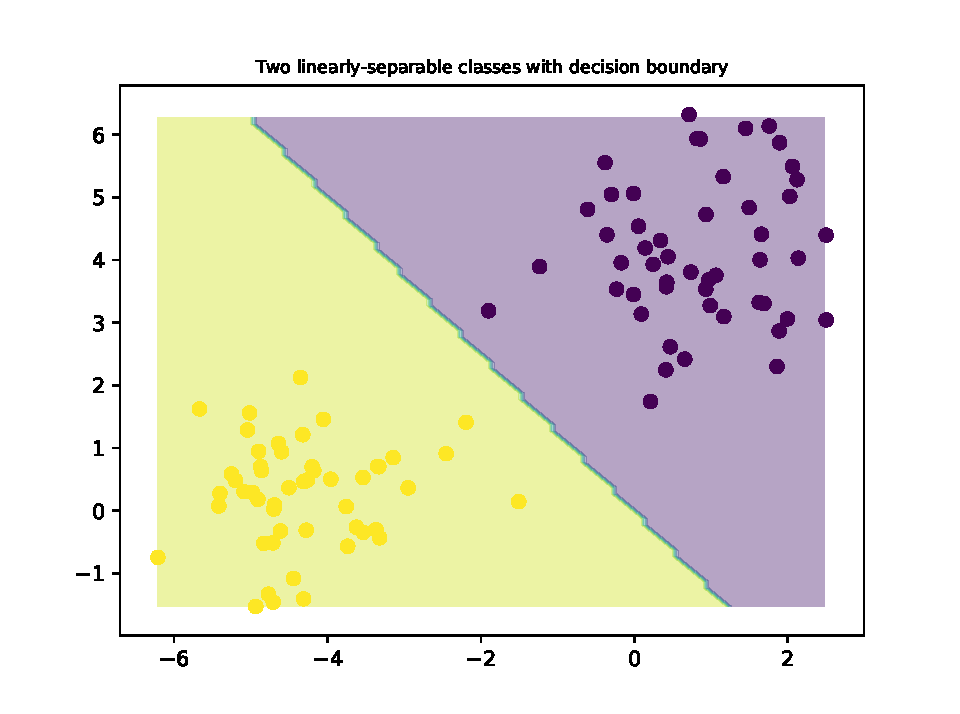
\includegraphics[width=\textwidth]{./Figures/3_lin_eta001_iter5.pdf}
	\caption{self implementation}
	\end{subfigure}
	\begin{subfigure}{0.45\textwidth}
	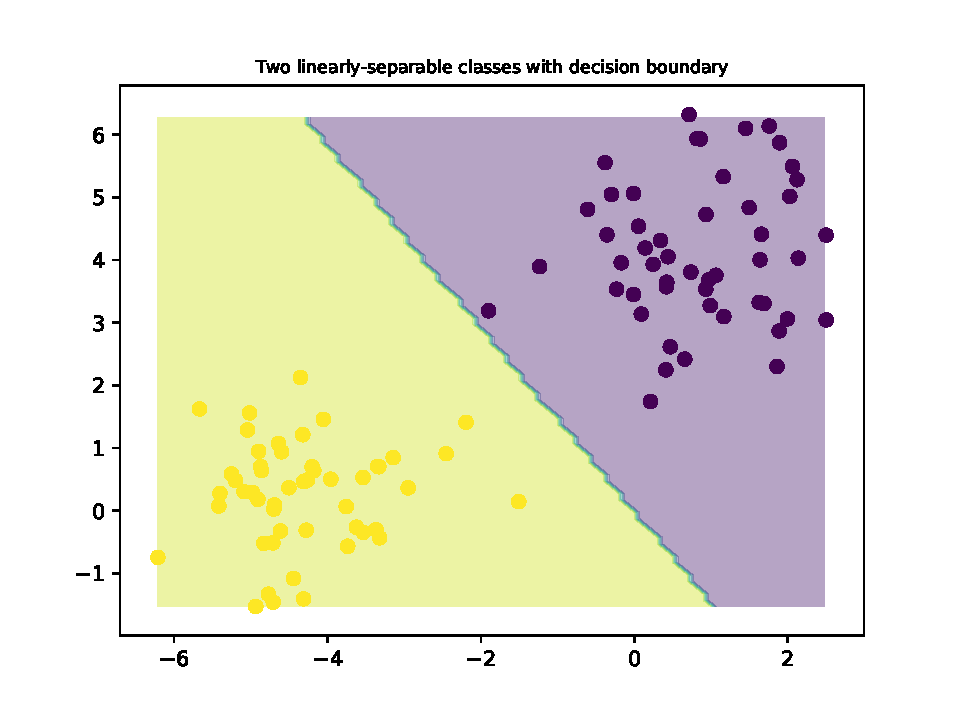
\includegraphics[width=\textwidth]{./Figures/3_lin_eta001_iter5_skl.pdf}
	\caption{scikit-learn’s implementation}
	\end{subfigure}
	}	
	\caption{Classification using eta = $0,01$ and max. iterations of 5}
	\label{perceptron2}
	\end{figure}
	
	\begin{figure}[!ht]
	\makebox[\textwidth]{
	\begin{subfigure}{0.45\textwidth}
	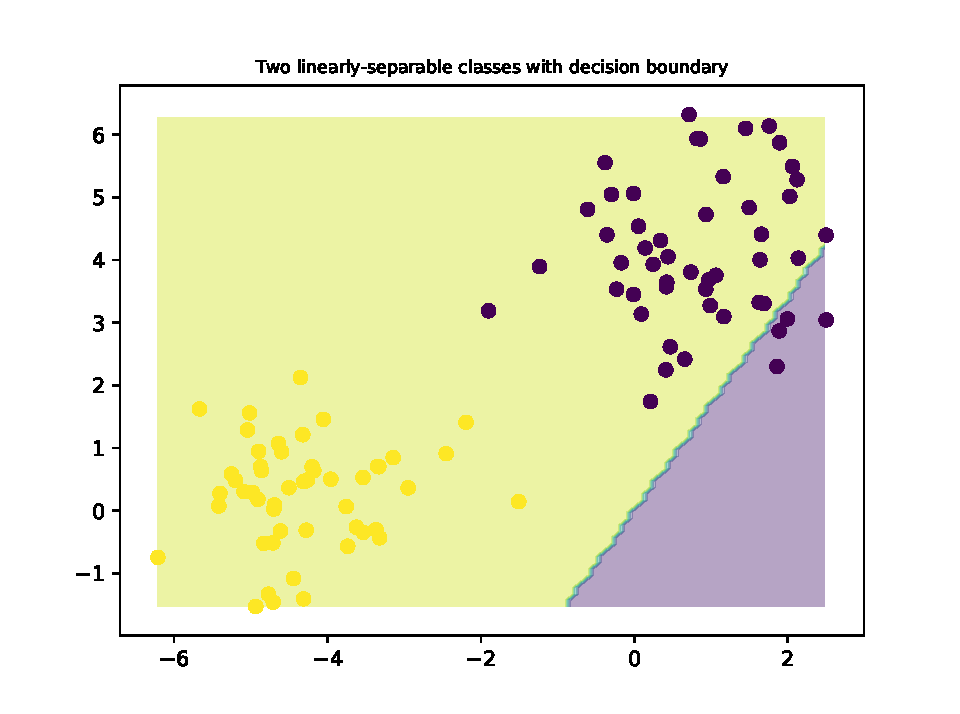
\includegraphics[width=\textwidth]{./Figures/3_lin_eta0001_iter5.pdf}
	\caption{self implementation}
	\end{subfigure}
	\begin{subfigure}{0.45\textwidth}
	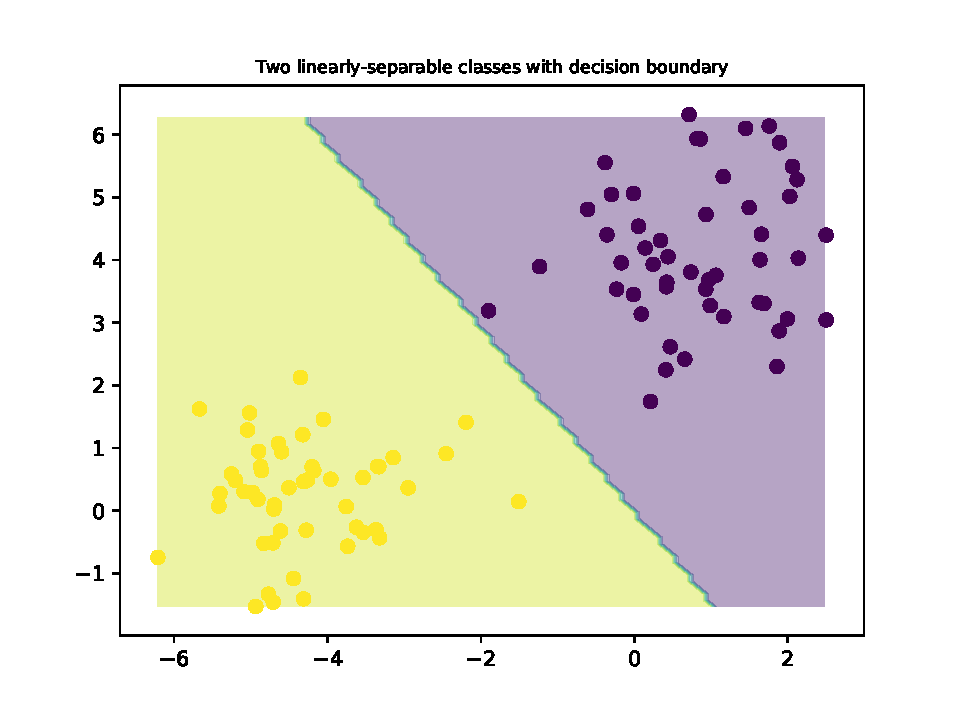
\includegraphics[width=\textwidth]{./Figures/3_lin_eta0001_iter5_skl.pdf}
	\caption{scikit-learn’s implementation}
	\end{subfigure}
	}	
	\caption{Classification using eta = $0,001$ and max. iterations of 5}
	\label{perceptron3}
	\end{figure}
	
	The classification of the dataset was similar for both implementations. Only using small eta's $< 0,001$ our code began  to misclassify the whole dataset.
	
	\item How many training iterations does it take for the perceptron to learn to classify all training samples perfectly?\\
	
	Our own implementation needs in average 2 iterations to classify the linear dataset perfectly. This make sense since we're using random initial weights for just two different states.\\
	
	
	\item The misclassification rate for both datasets
	
	\begin{table}[!ht]
	\parbox{.45\linewidth}{
	\centering
	\begin{tabular}{rc}
	\hline
	Training MSE: & 0,475 \\
	Test MSE: & 0,5 \\
	\hline
	\end{tabular}
	}
	\hfill
	\parbox{.45\linewidth}{
	\centering
	\begin{tabular}{rc}
	\hline
	Training MSE: & 0,475 \\
	Test MSE: & 0,5 \\
	\hline
	\end{tabular}
	\caption{MSEs using eta $= 0,01$ and 5 iterations self impl.(l.) skl.impl.(r.)}
	}
	\end{table}
	
	\begin{table}[!ht]
	\parbox{.45\linewidth}{
	\centering
	\begin{tabular}{rc}
	\hline
	Training MSE: & 0,525 \\
	Test MSE: & 0,55 \\
	\hline
	\end{tabular}
	}
	\hfill
	\parbox{.45\linewidth}{
	\centering
	\begin{tabular}{rc}
	\hline
	Training MSE: & 0,475 \\
	Test MSE: & 0,5 \\
	\hline
	\end{tabular}
	\caption{MSEs using eta $= 0,1$ and 100 iterations self impl.(l.) skl.impl.(r.)}
	}
	\end{table}
	
	\item Non linear seperable dataset:
	
	\begin{figure}[!ht]
	\makebox[\textwidth]{
	\begin{subfigure}{0.45\textwidth}
	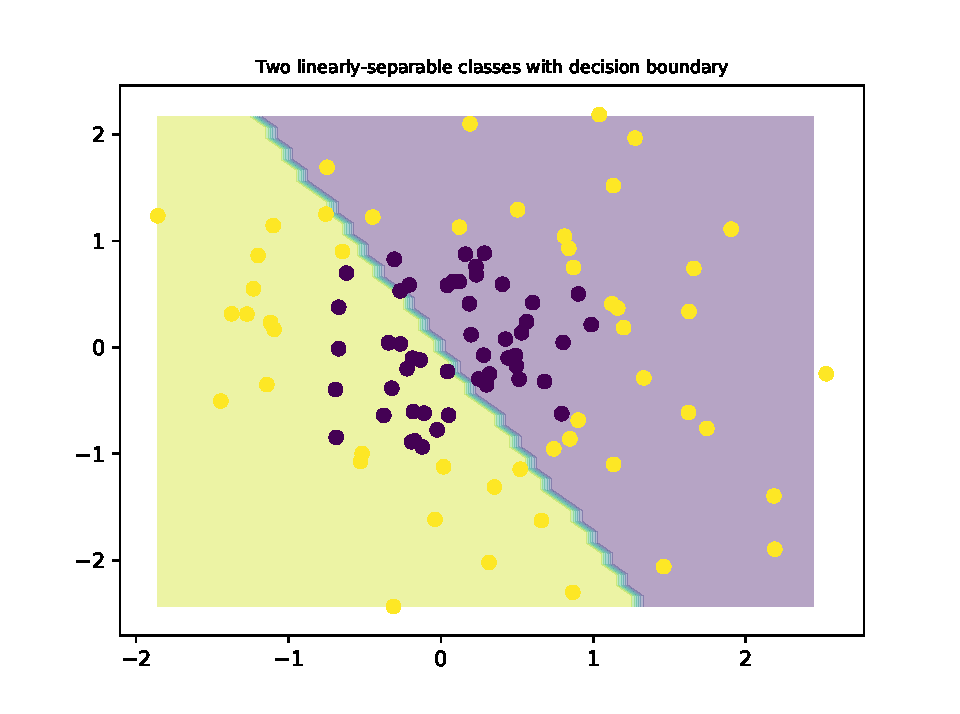
\includegraphics[width=\textwidth]{./Figures/3_nonlin_eta001_iter5.pdf}
	\caption{self implementation}
	\end{subfigure}
	\begin{subfigure}{0.45\textwidth}
	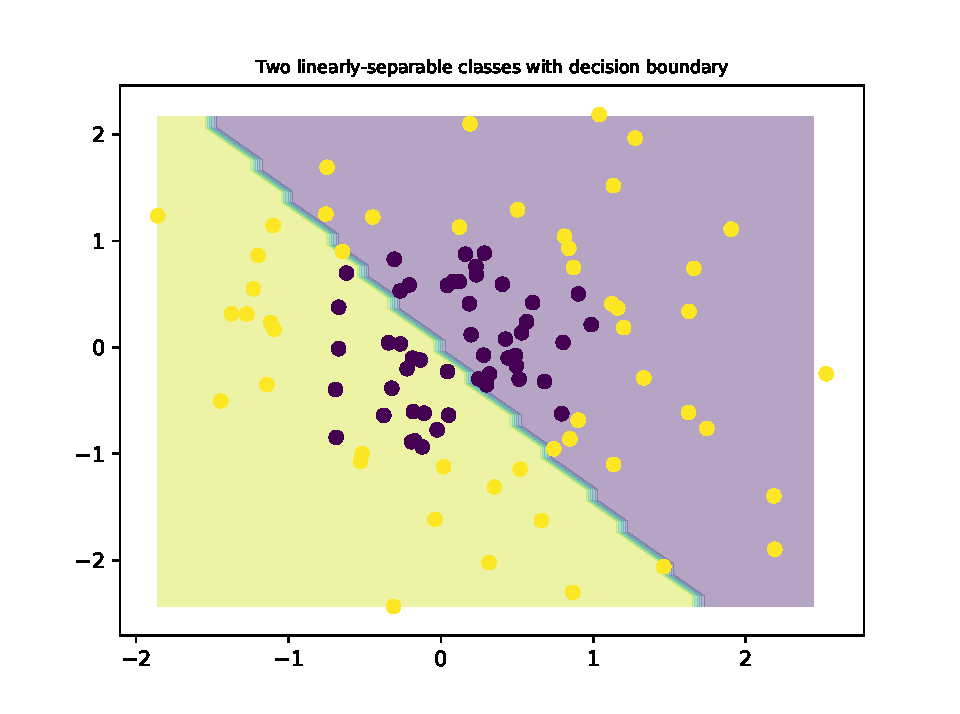
\includegraphics[width=\textwidth]{./Figures/3_nonlin_eta001_iter5_skl.pdf}
	\caption{scikit-learn’s implementation}
	\end{subfigure}
	}	
	\caption{Classification using eta = $0,01$ and max. iterations of 5}
	\label{perceptron1}
	\end{figure}
	
	\begin{figure}[!ht]
	\makebox[\textwidth]{
	\begin{subfigure}{0.45\textwidth}
	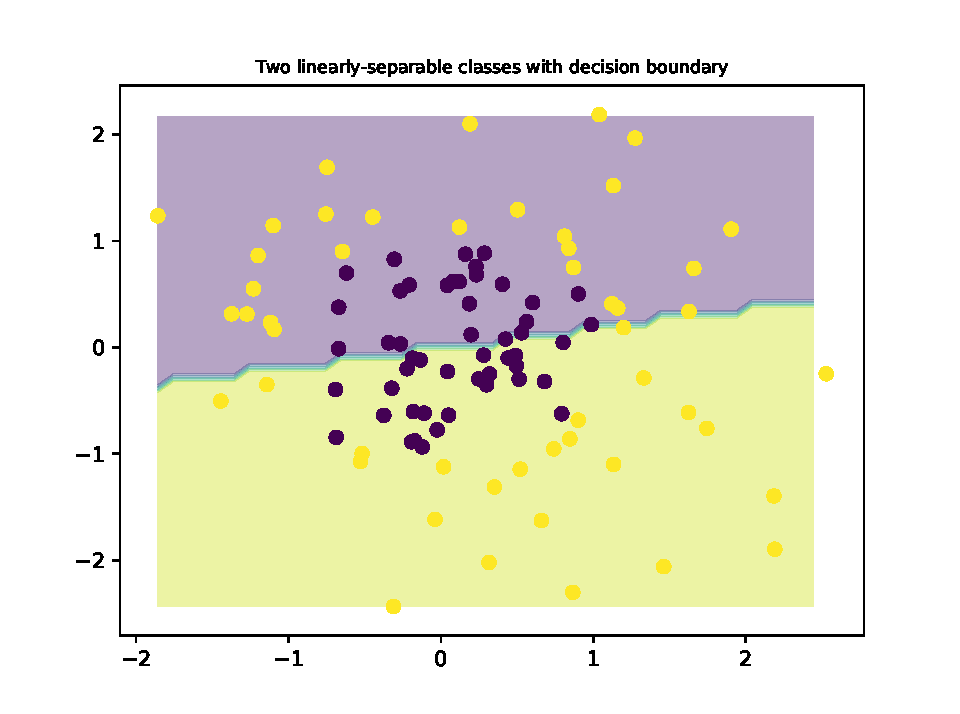
\includegraphics[width=\textwidth]{./Figures/3_nonlin_eta01_iter100.pdf}
	\caption{self implementation}
	\end{subfigure}
	\begin{subfigure}{0.45\textwidth}
	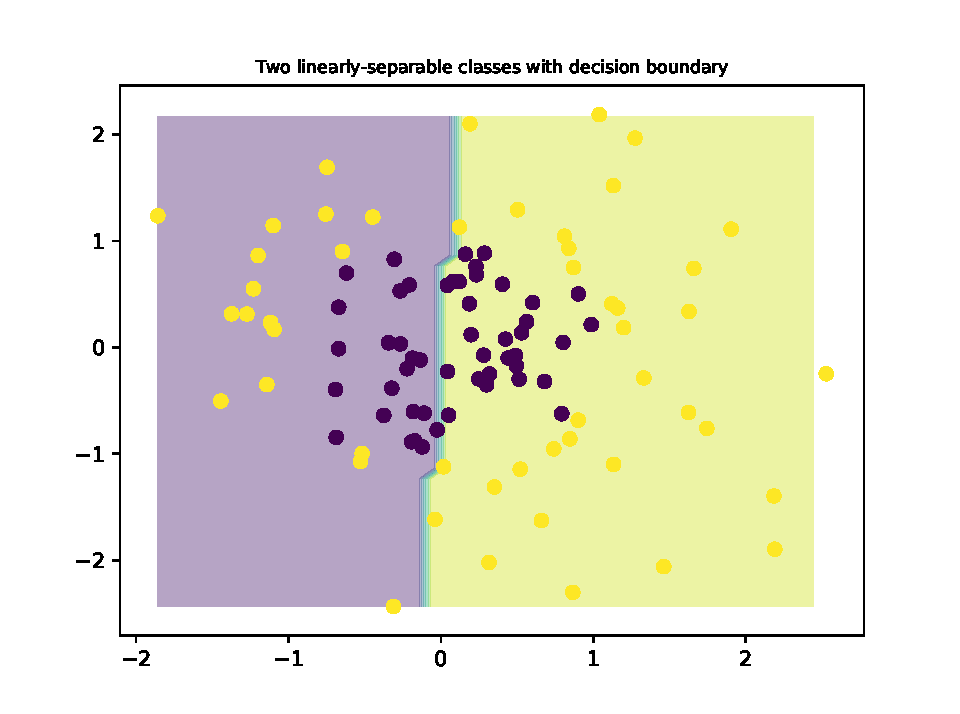
\includegraphics[width=\textwidth]{./Figures/3_nonlin_eta01_iter100_skl.pdf}
	\caption{scikit-learn’s implementation}
	\end{subfigure}
	}	
	\caption{Classification using eta = $0,1$ and max. iterations of 100}
	\label{perceptron2}
	\end{figure}

    Both implementations can not classify the non linear dataset.\\
    
    \item How would you learn a non-linear decision boundary using a single perceptron?\\
    
    We should use a non linear activation function i.e. the sigmoid function with logistic regression as we used it in our homework 2. Using a suiting degree and learning rate  the classification could be much better.
	
	
\end{itemize}

\end{document}}